\documentclass[journal,12pt,twocolumn]{IEEEtran}

\usepackage{setspace}
\usepackage{gensymb}
\singlespacing
\usepackage[cmex10]{amsmath}

\usepackage{amsthm}

\usepackage{mathrsfs}
\usepackage{txfonts}
\usepackage{stfloats}
\usepackage{bm}
\usepackage{cite}
\usepackage{cases}
\usepackage{subfig}

\usepackage{longtable}
\usepackage{multirow}

\usepackage{enumitem}
\usepackage{mathtools}
\usepackage{steinmetz}
\usepackage{tikz}
\usepackage{circuitikz}
\usepackage{verbatim}
\usepackage{tfrupee}
\usepackage[breaklinks=true]{hyperref}
\usepackage{graphicx}
\usepackage{tkz-euclide}

\usetikzlibrary{calc,math}
\usepackage{listings}
    \usepackage{color}                                            %%
    \usepackage{array}                                            %%
    \usepackage{longtable}                                        %%
    \usepackage{calc}                                             %%
    \usepackage{multirow}                                         %%
    \usepackage{hhline}                                           %%
    \usepackage{ifthen}                                           %%
    \usepackage{lscape}     
\usepackage{multicol}
\usepackage{chngcntr}

\DeclareMathOperator*{\Res}{Res}

\renewcommand\thesection{\arabic{section}}
\renewcommand\thesubsection{\thesection.\arabic{subsection}}
\renewcommand\thesubsubsection{\thesubsection.\arabic{subsubsection}}

\renewcommand\thesectiondis{\arabic{section}}
\renewcommand\thesubsectiondis{\thesectiondis.\arabic{subsection}}
\renewcommand\thesubsubsectiondis{\thesubsectiondis.\arabic{subsubsection}}


\hyphenation{op-tical net-works semi-conduc-tor}
\def\inputGnumericTable{}                                 %%

\lstset{
%language=C,
frame=single, 
breaklines=true,
columns=fullflexible
}
\begin{document}

\newcommand{\BEQA}{\begin{eqnarray}}
\newcommand{\EEQA}{\end{eqnarray}}
\newcommand{\define}{\stackrel{\triangle}{=}}
\bibliographystyle{IEEEtran}
\raggedbottom
\setlength{\parindent}{0pt}
\providecommand{\mbf}{\mathbf}
\providecommand{\pr}[1]{\ensuremath{\Pr\left(#1\right)}}
\providecommand{\qfunc}[1]{\ensuremath{Q\left(#1\right)}}
\providecommand{\sbrak}[1]{\ensuremath{{}\left[#1\right]}}
\providecommand{\lsbrak}[1]{\ensuremath{{}\left[#1\right.}}
\providecommand{\rsbrak}[1]{\ensuremath{{}\left.#1\right]}}
\providecommand{\brak}[1]{\ensuremath{\left(#1\right)}}
\providecommand{\lbrak}[1]{\ensuremath{\left(#1\right.}}
\providecommand{\rbrak}[1]{\ensuremath{\left.#1\right)}}
\providecommand{\cbrak}[1]{\ensuremath{\left\{#1\right\}}}
\providecommand{\lcbrak}[1]{\ensuremath{\left\{#1\right.}}
\providecommand{\rcbrak}[1]{\ensuremath{\left.#1\right\}}}
\theoremstyle{remark}
\newtheorem{rem}{Remark}
\newcommand{\sgn}{\mathop{\mathrm{sgn}}}
\providecommand{\abs}[1]{\vert#1\vert}
\providecommand{\res}[1]{\Res\displaylimits_{#1}} 
\providecommand{\norm}[1]{\lVert#1\rVert}
%\providecommand{\norm}[1]{\lVert#1\rVert}
\providecommand{\mtx}[1]{\mathbf{#1}}
\providecommand{\mean}[1]{E[ #1 ]}
\providecommand{\fourier}{\overset{\mathcal{F}}{ \rightleftharpoons}}
%\providecommand{\hilbert}{\overset{\mathcal{H}}{ \rightleftharpoons}}
\providecommand{\system}{\overset{\mathcal{H}}{ \longleftrightarrow}}
	%\newcommand{\solution}[2]{\textbf{Solution:}{#1}}
\newcommand{\solution}{\noindent \textbf{Solution: }}
\newcommand{\cosec}{\,\text{cosec}\,}
\providecommand{\dec}[2]{\ensuremath{\overset{#1}{\underset{#2}{\gtrless}}}}
\newcommand{\myvec}[1]{\ensuremath{\begin{pmatrix}#1\end{pmatrix}}}
\newcommand{\mydet}[1]{\ensuremath{\begin{vmatrix}#1\end{vmatrix}}}
\numberwithin{equation}{subsection}
\makeatletter
\@addtoreset{figure}{problem}
\makeatother
\let\StandardTheFigure\thefigure
\let\vec\mathbf
\renewcommand{\thefigure}{\theproblem}
\def\putbox#1#2#3{\makebox[0in][l]{\makebox[#1][l]{}\raisebox{\baselineskip}[0in][0in]{\raisebox{#2}[0in][0in]{#3}}}}
     \def\rightbox#1{\makebox[0in][r]{#1}}
     \def\centbox#1{\makebox[0in]{#1}}
     \def\topbox#1{\raisebox{-\baselineskip}[0in][0in]{#1}}
     \def\midbox#1{\raisebox{-0.5\baselineskip}[0in][0in]{#1}}
\vspace{3cm}
\title{ Gate-Assignment}
\author{Manikanta vallepu - AI20BTECH11014}
\maketitle
\newpage
\bigskip
\renewcommand{\thefigure}{\theenumi}
\renewcommand{\thetable}{\theenumi}
Download all python codes from 
\begin{lstlisting}
https://github.com/AI20BTECH11014/EE3900-Linear-Systems-and-Signal-processing/blob/main/Gate_assignment/Gate_assignment.py
\end{lstlisting}
%
and latex-tikz codes from 
%
\begin{lstlisting}
https://github.com/AI20BTECH11014/EE3900-Linear-Systems-and-Signal-processing/blob/main/Gate_assignment/Gate_assignment.tex
\vspace{0.5cm}
\section{QUESTION: Q.55 EC-GATE-2018}
\end{lstlisting}
  Let $X\sbrak{k}= k +1, 0 \leq k \leq 7$ be 8-point DFT of a sequence $x\sbrak{n}$,where$$X\sbrak{k}= \sum_{n=0}^{N-1} x\sbrak{n}e^{\dfrac{-j2\pi nk}{N}}$$
  The value (correct to two decimal places) of $\sum_{n=0}^{3} x[2n]$
\section{SOLUTION}

Given, $$X\sbrak{k}= \sum_{n=0}^{N-1} x\sbrak{n}e^{\dfrac{-j2\pi nk}{N}}$$
Considering 8-point DFT, we have 
\begin{align}
&\myvec{X\sbrak{0}\\X\sbrak{1}\\X\sbrak{2}\\X\sbrak{3}\\X\sbrak{4}\\X\sbrak{5}\\X\sbrak{6}\\X\sbrak{7}} = \myvec{W_{8}^{0}&W_{8}^{0}&W_{8}^{0}&W_{8}^{0}&W_{8}^{0}&W_{8}^{0}&W_{8}^{0}&W_{8}^{0}\\W_{8}^{0}&W_{8}^{1}&W_{8}^{2}&W_{8}^{3}&W_{8}^{4}&W_{8}^{5}&W_{8}^{6}&W_{8}^{7}\\W_{8}^{0}&W_{8}^{2}&W_{8}^{4}&W_{8}^{6}&W_{8}^{8}&W_{8}^{10}&W_{8}^{12}&W_{8}^{14}\\W_{8}^{0}&W_{8}^{3}&W_{8}^{6}&W_{8}^{9}&W_{8}^{12}&W_{8}^{15}&W_{8}^{18}&W_{8}^{21}\\W_{8}^{0}&W_{8}^{4}&W_{8}^{8}&W_{8}^{12}&W_{8}^{16}&W_{8}^{20}&W_{8}^{24}&W_{8}^{28}\\W_{8}^{0}&W_{8}^{5}&W_{8}^{10}&W_{8}^{15}&W_{8}^{20}&W_{8}^{25}&W_{8}^{30}&W_{8}^{35}\\W_{8}^{0}&W_{8}^{6}&W_{8}^{12}&W_{8}^{18}&W_{8}^{24}&W_{8}^{30}&W_{8}^{36}&W_{8}^{42}\\W_{8}^{0}&W_{8}^{7}&W_{8}^{14}&W_{8}^{21}&W_{8}^{28}&W_{8}^{35}&W_{8}^{42}&W_{8}^{49}}\myvec{x\sbrak{0}\\x\sbrak{1}\\x\sbrak{2}\\x\sbrak{3}\\x\sbrak{4}\\x\sbrak{5}\\x\sbrak{6}\\x\sbrak{7}} \label{eq:1}\\
&\text{where twiddler factor}, W_{8} = \text{exp}\brak{-\frac{j2\pi}{8}} \label{eq:2}
\end{align}
Obtaining X\sbrak{0} and X\sbrak{4} by using \eqref{eq:2}, we get,
\begin{align}
X\sbrak{0}={}&\myvec{1&1&1&1&1&1&1&1}\myvec{x\sbrak{0}\\x\sbrak{1}\\x\sbrak{2}\\x\sbrak{3}\\x\sbrak{4}\\x\sbrak{5}\\x\sbrak{6}\\x\sbrak{7}} \label{eq:3}\\
X\sbrak{4}={}&\myvec{1&-1&1&-1&1&-1&1&-1}\myvec{x\sbrak{0}\\x\sbrak{1}\\x\sbrak{2}\\x\sbrak{3}\\x\sbrak{4}\\x\sbrak{5}\\x\sbrak{6}\\x\sbrak{7}} \label{eq:4}
\end{align}
from \eqref{eq:3} and \eqref{eq:4},
\begin{align}
X\sbrak{0} + X\sbrak{4}={}&\myvec{2&0&2&0&2&0&2&0}\myvec{x\sbrak{0}\\x\sbrak{1}\\x\sbrak{2}\\x\sbrak{3}\\x\sbrak{4}\\x\sbrak{5}\\x\sbrak{6}\\x\sbrak{7}} 
\end{align}
\newpage 
\begin{align}
X\sbrak{0} + X\sbrak{4}&=2\brak{ x\sbrak{0} + x\sbrak{2} +x\sbrak{4} + x\sbrak{6}}\\
X\sbrak{0} + X\sbrak{4}&=2\sum_{n=0}^{3} x\sbrak{2n} \label{eq:5}
\end{align}
given,
\begin{align}
    X\sbrak{k}= k +1, 0 \leq k \leq 7 \label{eq:6}
\end{align}
from \eqref{eq:5} and \eqref{eq:6},
\begin{align}
   \sum_{n=0}^{3} x\sbrak{2n} = 3
\end{align}
\begin{figure}[!ht]
    \centering
    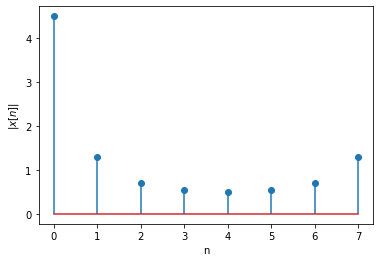
\includegraphics[width=\columnwidth] {fig.png}
    \caption{Magnitude of $x\sbrak{n}$ vs $n$}
\end{figure}
\end{document}
